\subsubsection{Configurazione tempi di ricalcolo}
\begin{figure} [H]
	\centering
	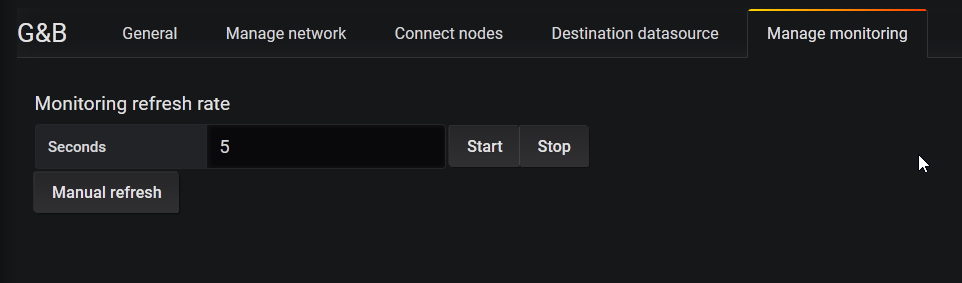
\includegraphics[scale=0.55]{Img/monitoring} 
	\caption{Tab di configurazione tempi di ricalcolo} \label{} 
\end{figure} 
Dopo aver scelto la datasource e il database in cui scrivere il risultato del processo di ricalcolo delle probabilità dei nodi della rete, avrete la possibilità di scegliere in che modo effettuare il monitoraggio:
\begin{itemize}
	\item Saltuariamente tramite il tasto "\emph{Ricalcola}";
	\item Costantemente, utilizzando i tasti "\emph{Start}" e "\emph{Stop}" e la cella di testo in cui specificare, in secondi, il timer di refresh. L'iter per il corretto settaggio è il seguente:
		\begin{enumerate}
				\item Settare il timer di ricalcolo (in secondi e con un numero >=0);
				\item Cliccare sul pulsante "\emph{Start}" per iniziare il monitoraggio;
				\item Cliccare sul pulsante "\emph{Stop}" per terminare il ricalcolo.
		\end{enumerate}
\end{itemize}